% =============================================================
%  Excel Transfer Tool — Premium User Manual
%  Modern, professional LaTeX layout
% =============================================================
\documentclass[11pt,a4paper]{article}

% ── Core layout ──────────────────────────────────────────────
\usepackage[a4paper,top=2.8cm, bottom=3cm,left=2.4cm, right=2.4cm,headheight=14pt]{geometry}

% ── Typography ───────────────────────────────────────────────
\usepackage[T1]{fontenc}
\usepackage[utf8]{inputenc}
\usepackage{lmodern}
\usepackage{microtype}
\usepackage{setspace}
\usepackage{letterspace}  % For \textls letter spacing
\setstretch{1.15}

% ── Graphics & color ─────────────────────────────────────────
\usepackage{graphicx}
\usepackage{float}
\usepackage[table]{xcolor}
\usepackage{tikz}
\usetikzlibrary{shadows.blur, positioning, shapes.geometric}

% ── Header / footer ──────────────────────────────────────────
\usepackage{fancyhdr}
\usepackage{lastpage}

% ── Tables ───────────────────────────────────────────────────
\usepackage{booktabs}
\usepackage{tabularx}
\usepackage{array}

% ── Lists ────────────────────────────────────────────────────
\usepackage{enumitem}

% ── Sections styling ─────────────────────────────────────────
\usepackage{titlesec}

% ── Colored boxes ────────────────────────────────────────────
\usepackage{etoolbox}
\usepackage[most]{tcolorbox}

% ── Hyperlinks ───────────────────────────────────────────────
\usepackage{hyperref}

% ── Misc ─────────────────────────────────────────────────────
\usepackage{parskip}
\usepackage{mdframed}

% =============================================================
%  COLOUR PALETTE - Light Premium Professional
% =============================================================
\definecolor{PrimaryBlue}{HTML}{2C3E50}      % Deep slate - serious but not dark
\definecolor{AccentBlue}{HTML}{5D6D7E}       % Muted blue-gray
\definecolor{LightBlue}{HTML}{EBF5FB}        % Very light blue
\definecolor{Teal}{HTML}{7D8A96}             % Soft teal-gray
\definecolor{LightTeal}{HTML}{E8F0F5}        % Pale blue
\definecolor{SoftGray}{HTML}{F8F9FA}         % Off-white
\definecolor{MidGray}{HTML}{D5DBDB}          % Light gray
\definecolor{DarkText}{HTML}{34495E}         % Charcoal blue
\definecolor{MutedText}{HTML}{85929E}        % Soft gray
\definecolor{Warning}{HTML}{D68910}          % Warm amber
\definecolor{LightWarning}{HTML}{FEF9E7}     % Pale yellow
\definecolor{Danger}{HTML}{CB4335}           % Muted red
\definecolor{Success}{HTML}{27AE60}          % Fresh green
\definecolor{LightSuccess}{HTML}{EAFAF1}     % Pale green
\definecolor{White}{HTML}{FFFFFF}
\definecolor{PremiumGold}{HTML}{D4AF37}      % Elegant gold
\definecolor{ModernBlue}{HTML}{3498DB}       % Clean modern blue
\definecolor{SoftPurple}{HTML}{9B59B6}       % Elegant purple
\definecolor{LightAccent}{HTML}{F4F6F7}      % Almost white with hint of blue

% =============================================================
%  HYPERREF SETUP
% =============================================================
\hypersetup{
    colorlinks=true,
    linkcolor=AccentBlue,
    urlcolor=Teal,
    citecolor=AccentBlue,
    pdftitle={Excel Transfer Tool User Manual},
    pdfauthor={Finance Automation Team},
    bookmarksnumbered=true
}

% =============================================================
%  HEADER & FOOTER
% =============================================================
\pagestyle{fancy}
\fancyhf{}
\fancyhead[L]{%
    
\begin{tikzpicture}[baseline=(A.base)]
        \node[inner sep=0pt] (A) {%
            \textcolor{PrimaryBlue}{\textbf{\small Excel Transfer Tool}}%
        };
    \end{tikzpicture}%
}
\fancyhead[C]{\textcolor{MutedText}{\small User Manual}}
\fancyhead[R]{\textcolor{MutedText}{\small v2.0 · \today}}

\renewcommand{\headrulewidth}{0.4pt}
\renewcommand{\headrule}{\hbox to\headwidth{%
    \color{AccentBlue}\leaders\hrule height \headrulewidth\hfill}}

\fancyfoot[L]{\textcolor{MutedText}{\scriptsize Finance Automation · Internal Use Only}}
\fancyfoot[C]{}
\fancyfoot[R]{\textcolor{MutedText}{\scriptsize Page \thepage\ of \pageref{LastPage}}}

\renewcommand{\footrulewidth}{0.4pt}
\renewcommand{\footrule}{\hbox to\headwidth{%
    \color{MidGray}\leaders\hrule height \footrulewidth\hfill}}

% =============================================================
%  SECTION STYLING
% =============================================================
\titleformat{\section}{%
    \Large\bfseries\color{White}%
}{}{0em}{%
    \colorbox{PrimaryBlue}{\parbox{\dimexpr\linewidth-2\fboxsep\relax}{%
        \vspace{4pt}\hspace{6pt}%
        \Large\bfseries\color{White}%
    }}%
}

\titleformat{\subsection}{%
    \large\bfseries\color{PrimaryBlue}%
}{}{0em}{%
    \large\bfseries\color{PrimaryBlue}%
}[\vspace{-6pt}\textcolor{AccentBlue}{\rule{\linewidth}{1.5pt}}]

\titleformat{\subsubsection}{%
    \normalsize\bfseries\color{AccentBlue}%
}{}{0em}{}

% =============================================================
%  CUSTOM BOXES
% =============================================================
% Info box
\newtcolorbox{infobox}[1][Note]{
    enhanced,
    colback=LightBlue,
    colframe=AccentBlue,
    boxrule=1pt,
    arc=6pt,
    left=10pt, right=10pt, top=8pt, bottom=8pt,
    fonttitle=\bfseries\color{AccentBlue},
    title=#1,
    attach boxed title to top left={yshift=-2mm, xshift=6mm},
    boxed title style={colback=LightBlue, colframe=AccentBlue, arc=4pt}
}

% Warning box
\newtcolorbox{warningbox}[1][Warning]{
    enhanced, colback=LightWarning, colframe=Warning, boxrule=1pt, arc=6pt,
    left=10pt, right=10pt, top=8pt, bottom=8pt,
    fonttitle=\bfseries\color{Warning}, title=#1,
    attach boxed title to top left={yshift=-2mm, xshift=6mm},
    boxed title style={colback=LightWarning, colframe=Warning, arc=4pt}
}

% Success box
\newtcolorbox{successbox}[1][Success]{
    enhanced, colback=LightSuccess, colframe=Success, boxrule=1pt, arc=6pt,
    left=10pt, right=10pt, top=8pt, bottom=8pt,
    fonttitle=\bfseries\color{Success}, title=#1,
    attach boxed title to top left={yshift=-2mm, xshift=6mm},
    boxed title style={colback=LightSuccess, colframe=Success, arc=4pt}
}

% Step box
\newtcolorbox{stepbox}[1][]{
    enhanced, colback=SoftGray, colframe=MidGray, boxrule=0.8pt, arc=8pt,
    left=12pt, right=12pt, top=10pt, bottom=10pt,
    drop shadow={SoftGray!80!black}, #1
}

% Code / path box
\newtcolorbox{codebox}{
    enhanced, colback=DarkText, colframe=DarkText, boxrule=0pt, arc=4pt,
    left=10pt, right=10pt, top=6pt, bottom=6pt,
    fontupper=\ttfamily\small\color{White}
}

% Screenshot placeholder
\newcommand{\screenshot}[3][8cm]{%
\begin{figure}[H]
\centering
\begin{tikzpicture}
\node[draw=MidGray,fill=SoftGray,rounded corners=8pt,minimum width=0.88\linewidth,
      minimum height=#1,drop shadow={shadow xshift=2pt, shadow yshift=-2pt, opacity=0.15},
      align=center,font=\color{MutedText}\small] {%
    \begin{minipage}{0.75\linewidth}
    \centering\vspace{0.5cm}
    \begin{tikzpicture}
    \node[draw=MidGray, fill=MidGray, rounded corners=4pt,
          minimum width=1.2cm, minimum height=0.8cm]{};
    \end{tikzpicture}\\[6pt]
    \textcolor{MutedText}{\textit{#2}}
    \end{minipage}};
\end{tikzpicture}
\caption{#3}
\label{fig:#3}
\end{figure}}


% ── v3.0 additions ─────────────────────────────────────────────
\definecolor{NewFeature}{HTML}{1A5276}
\definecolor{LightNew}{HTML}{D6EAF8}
\newtcolorbox{newbox}[1][New in v1.0]{
  colback=LightNew, colframe=NewFeature, coltitle=White,
  fonttitle=\bfseries\small, title=\textbf{*}\ #1, arc=4pt,
  left=8pt, right=8pt, top=6pt, bottom=6pt
}
\begin{document}

 Title Page 
\begin{titlepage}
\newgeometry{margin=0pt}
\begin{tikzpicture}[remember picture, overlay]
\fill[White] (current page.north west) rectangle (current page.south east);
\begin{scope}[transparency group, opacity=0.08]
\fill[ModernBlue] ([xshift=-6cm, yshift=-2cm]current page.north east) circle (4cm);
\fill[SoftPurple]  ([xshift=-3cm, yshift=-5cm]current page.north east) circle (3cm);
\end{scope}
\begin{scope}[transparency group, opacity=0.06]
\fill[PremiumGold] ([xshift=2cm, yshift=-8cm]current page.north west) -- ([xshift=5cm, yshift=-8cm]current page.north west) -- ([xshift=3.5cm, yshift=-12cm]current page.north west) -- cycle;
\fill[ModernBlue]  ([xshift=1cm, yshift=-14cm]current page.north west) rectangle ([xshift=4cm, yshift=-17cm]current page.north west);
\end{scope}
\begin{scope}[transparency group, opacity=0.12]
\fill[PremiumGold] ([xshift=1cm, yshift=-2cm]current page.north west) rectangle ([xshift=1.8cm, yshift=-2.8cm]current page.north west);
\fill[ModernBlue]  ([xshift=2cm, yshift=-2cm]current page.north west) rectangle ([xshift=2.8cm, yshift=-2.8cm]current page.north west);
\fill[SoftPurple]  ([xshift=3cm, yshift=-2cm]current page.north west) rectangle ([xshift=3.8cm, yshift=-2.8cm]current page.north west);
\end{scope}
\fill[PremiumGold, opacity=0.4] ([xshift=0.8cm, yshift=-4cm]current page.north west) rectangle ([xshift=0.9cm, yshift=-10cm]current page.north west);
\fill[LightAccent] (current page.north west) rectangle ([yshift=-0.3cm]current page.north east);
\end{tikzpicture}

\vspace*{6cm}
\begin{center}

\begin{tikzpicture}
\fill[PremiumGold, opacity=0.7] (0,0) rectangle (0.8,0.8);
\fill[ModernBlue,  opacity=0.6] (1,0) rectangle (1.8,0.8);
\fill[SoftPurple,  opacity=0.5] (2,0) rectangle (2.8,0.8);
\fill[NewFeature,  opacity=0.7] (3.2,0) rectangle (4.0,0.8);
\end{tikzpicture}

\vspace{1.5cm}
{\fontsize{44}{52}\selectfont\color{PrimaryBlue}\textls[120]{\textbf{EXCEL TRANSFER TOOL}}}\\[1cm]
{\fontsize{13}{16}\selectfont\color{AccentBlue}\textsc{Technical Documentation \& User Guide}}\\[0.5cm]

\begin{tikzpicture}
\draw[PremiumGold, line width=1.5pt] (0,0) -- (3,0);
\fill[ModernBlue, opacity=0.6] (3.3,-0.15) rectangle (3.6,0.15);
\fill[NewFeature,  opacity=0.7] (3.7,-0.15) rectangle (4.0,0.15);
\draw[ModernBlue, line width=1pt, opacity=0.5] (4.2,0) -- (5.5,0);
\end{tikzpicture}

\vspace{0.8cm}
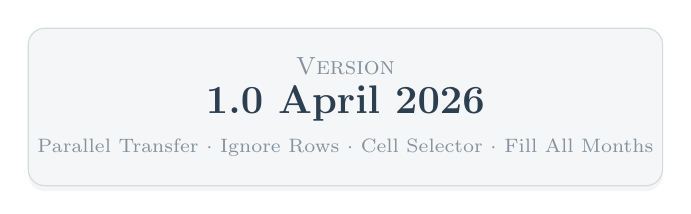
\begin{tikzpicture}
\node[draw=MidGray,fill=LightAccent,rounded corners=6pt,
      minimum width=7cm,minimum height=2cm,align=center,
      drop shadow={shadow xshift=0pt,shadow yshift=-2pt,opacity=0.08}] {%
  {\small\color{MutedText}\textsc{Version}}\\[2pt]
  {\Large\color{PrimaryBlue}\textbf{1.0 April 2026}}\\[2pt]
  {\scriptsize\color{MutedText}Parallel Transfer $\cdot$ Ignore Rows $\cdot$ Cell Selector $\cdot$ Fill All Months}
};
\end{tikzpicture}

\vspace{2.5cm}

\begin{tikzpicture}
\node[draw=ModernBlue,fill=LightBlue,rounded corners=12pt,minimum width=2.5cm,minimum height=0.8cm,align=center] at (0,0) {\small\color{PrimaryBlue}\textbf{Qt 6}};
\node[draw=SoftPurple,fill=White,rounded corners=12pt,minimum width=2.8cm,minimum height=0.8cm,align=center] at (3.2,0) {\small\color{PrimaryBlue}\textbf{C++17}};
\node[draw=PremiumGold,fill=LightAccent,rounded corners=12pt,minimum width=3.2cm,minimum height=0.8cm,align=center] at (6.8,0) {\small\color{PrimaryBlue}\textbf{OpenXML}};
\node[draw=NewFeature,fill=LightNew,rounded corners=12pt,minimum width=3.5cm,minimum height=0.8cm,align=center] at (10.8,0) {\small\color{NewFeature}\textbf{Multi-Thread}};
\end{tikzpicture}

\vspace{3cm}
{\small\color{MutedText}Finance Automation Team \textbullet\ Internal Use Only}
\end{center}
\restoregeometry
\end{titlepage}

\newpage
\thispagestyle{fancy}
{\hypersetup{linkcolor=DarkText}
\setcounter{tocdepth}{1}
{\small\tableofcontents}}
\newpage

% =============================================================
\section{Overview}
% =============================================================

Excel Transfer Tool is a high-performance Qt/C++ desktop application that automates monthly cost-control reporting workflows. It loads Excel workbooks (XLSM/XLSX) for multiple periods, applies configurable transfer mappings, consolidates data across months, and produces clean output files---all without manual copy-paste work.

\begin{infobox}[Key Capabilities --- v1.0]
\begin{itemize}[leftmargin=*, itemsep=2pt]
\item Load multiple cost-control files with parallel processing (2-3x faster)
\item Apply row-level transfer mappings per month/sheet/column
\item Rolling Transfer (RT) mode for sequential month-to-month workflows
\item Parallel Transfer --- run Individual or Rolling modes from a unified backend
\item Fill All Months --- backfill Jan through target month in one operation
\item Ignore Rows --- skip specific rows per mapping card
\item Create Month File --- generate new month files from existing templates
\item Visual Cell Selector --- pick source/destination cells from a grid view
\item Log Panel toggle --- show/hide the status log on demand
\item Quarter quick-select buttons (Q1--Q4) for rapid period selection
\item Automatic formula preservation and shared formula handling
\end{itemize}
\end{infobox}

% ====================================================\dfrac{v1}{den}=========
\section{What's New in v1.0}
% =============================================================

\begin{center}
\rowcolors{2}{SoftGray}{White}
\begin{tabularx}{0.92\linewidth}{@{} l X @{}}
\toprule
\rowcolor{NewFeature}
\textcolor{White}{\textbf{Feature}} & \textcolor{White}{\textbf{Description}} \\
\midrule
Parallel Transfer Backend & New \texttt{ParallelTransferController} with \texttt{IndividualTransferWorker} and \texttt{RollingTransferWorker}. Each worker owns its own \texttt{ExcelHandler} and \texttt{TransferService} --- fully thread-safe. \\
Fill All Months & Writes Jan through target month into a single cost-control file. Destination always points to the \texttt{test/} subfolder. \\
Ignore Rows Dialog & Per-mapping-card dialog showing all rowMap entries. Check rows to skip during transfer. Filter by row number or value. \\
Create Month File & Button on each YearCard. Activates creation mode: select months, click Load Periods, app finds last existing file and copies it for missing months. \\
Visual Cell Selector & ``Select Source/Dest Cells'' opens a scrollable grid of the loaded Excel sheet. Click any cell to capture its reference. \\
Log Panel Toggle & ``Log'' button in header shows/hides the status log dock. Hidden by default on startup. \\
Copy Full Sheet hidden & For REFI/Budget/prev-year mappings (same-file sources), ``Copy full sheet'' is automatically hidden. \\
Run/Remove buttons removed & Mapping row cards no longer show Run and Remove buttons. \\
Toast positioning fixed & Blue notification toasts now appear at the bottom-center of the application window, not the screen. \\
\bottomrule
\end{tabularx}
\end{center}

% =============================================================
\section{Installation}
% =============================================================

\subsection{System Requirements}

\begin{center}
\rowcolors{2}{SoftGray}{White}
\begin{tabularx}{0.88\linewidth}{@{} l X @{}}
\toprule
\rowcolor{PrimaryBlue}
\textcolor{White}{\textbf{Component}} & \textcolor{White}{\textbf{Requirement}} \\
\midrule
Operating System & Windows 10 or Windows 11 (64-bit) \\
Microsoft Excel  & Excel 2016, 2019, 2021, or Microsoft 365 \\
Runtime          & Qt 6.x (bundled with executable) \\
Disk Space       & Minimum 200 MB free \\
RAM              & 8 GB minimum, 16 GB recommended for 12+ months \\
\bottomrule
\end{tabularx}
\end{center}

\subsection{Setup Steps}

\begin{stepbox}
\begin{enumerate}[leftmargin=*, itemsep=6pt]
\item Extract the application folder to your preferred location.
\item Ensure \texttt{repair.ps1} is in the same folder as \texttt{ExcelTransfer.exe}.
\item Launch \texttt{ExcelTransfer.exe}.
\item Verify the default folder paths point to your network share (L: drive).
\item Ensure cost-control files follow the expected naming convention.
\item Verify JSON mapping files exist in the \texttt{JSON/} subfolder.
\end{enumerate}
\end{stepbox}


% =============================================================
\section{User Interface}
% =============================================================

\begin{figure}[h]
\centering
\includegraphics[width=0.82\linewidth]{../../Pictures/Figure1.png}
\caption{Excel Transfer Tool --- Main window showing the Monthly Transfer tab with collapsed year cards.}
\label{fig:mainui}
\end{figure}

\subsection{Header Bar}

The header bar contains global controls:

\begin{center}
\rowcolors{2}{SoftGray}{White}
\begin{tabularx}{0.88\linewidth}{@{} l X @{}}
\toprule
\rowcolor{PrimaryBlue}
\textcolor{White}{\textbf{Button}} & \textcolor{White}{\textbf{Action}} \\
\midrule
Reset          & Clears all loaded files, mapping cards, and period rows \\
Create Month File & Opens creation mode on the year cards (see Section~\ref{sec:createmonth}) \\
Log            & Toggles the status log panel (hidden by default) \\
\bottomrule
\end{tabularx}
\end{center}

\subsection{Year Cards}

Each year card shows month checkboxes and quick-select controls:

\begin{itemize}[leftmargin=*, itemsep=4pt]
\item \textbf{Year checkbox} --- expands/collapses the card
\item \textbf{Q1--Q4 buttons} --- select/deselect entire quarters
\item \textbf{All / None} --- select or deselect all 12 months
\item \textbf{+ Create Files} --- activates file creation mode (amber button, appears when card is expanded)
\end{itemize}

\begin{figure}[h]
\centering
\includegraphics[width=0.82\linewidth]{../../Pictures/Figure4.png}
\caption{Year card expanded showing month checkboxes. July, August and September are selected (blue). Q1--Q4, All, and None quick-select buttons are visible on the right.}
\label{fig:yearcard}
\end{figure}

\begin{infobox}[Period Limit]
Maximum \textbf{5 months} can be selected at a time for Execute All. Selecting more shows a warning and prevents execution to avoid memory overflow.
\end{infobox}

\begin{figure}[h]
\centering
\includegraphics[width=0.82\linewidth]{../../Pictures/Figure6.png}
\caption{Individual Transfer tab showing the \textbf{Log} button in the header bar (top right). The status bar at the bottom displays live transfer progress.}
\label{fig:logbutton}
\end{figure}

\subsection{Log Panel}

Click the \textbf{Log} button in the header to show or hide the status log dock. The log panel is hidden by default on startup. When visible, it shows all transfer status, warnings, and debug output in real time.

% =============================================================
\section{Loading Files}
% =============================================================

\subsection{Selecting Periods}

\begin{stepbox}
\begin{enumerate}[leftmargin=*, itemsep=6pt]
\item Check the year checkbox (e.g.\ 2025) to expand the year card.
\item Select months individually or use Q1--Q4 / All / None buttons.
\item Click \textbf{LOAD Selected Periods}.
\item Wait for the green ``Loaded'' toast notification.
\end{enumerate}
\end{stepbox}

\begin{warningbox}[Important]
Ensure all target files are \textbf{closed in Excel} before loading. Open files cause ZIP read errors.
\end{warningbox}

% =============================================================
\section{Mapping Cards}
% =============================================================

\subsection{What is a Mapping Card?}

Each mapping card represents a transfer rule:

\begin{itemize}[leftmargin=*, itemsep=2pt]
\item A \textbf{source} workbook, sheet, and column
\item A \textbf{destination} sheet and column
\item A \textbf{rowMap} defining source row $\rightarrow$ destination row pairs
\end{itemize}

\subsection{Mapping Card Buttons}

\begin{center}
\rowcolors{2}{SoftGray}{White}
\begin{tabularx}{0.88\linewidth}{@{} l X @{}}
\toprule
\rowcolor{PrimaryBlue}
\textcolor{White}{\textbf{Button}} & \textcolor{White}{\textbf{Action}} \\
\midrule
Edit Rows    & Modify source/destination row numbers \\
Export       & Export rowMap to JSON file \\
Import       & Import rowMap from JSON file \\
\textcolor{Warning}{\textbf{{\small $\oslash$} Ignore}} & Open Ignore Rows dialog to skip specific rows \\
\bottomrule
\end{tabularx}
\end{center}

\begin{figure}[h]
\centering
\includegraphics[width=0.82\linewidth]{../../Pictures/Figure7.png}
\caption{Active Mappings section showing a loaded mapping card (SAP Report $\rightarrow$ MZLZ Consolidated). The card shows Src/Dest Sheet, Src/Dest Column, and action buttons: \textbf{Edit Rows}, \textbf{Export RowMap}, \textbf{Import RowMap}, and \textbf{Ignore}. The \textbf{+ Create Files} button is visible on the year card header.}
\label{fig:mappingcard}
\end{figure}

\begin{infobox}[Copy Full Sheet]
The ``Copy full sheet'' checkbox is \textbf{automatically hidden} for REFI, Budget, and prev-year mappings. These mappings read from the same cost-control file --- copying a sheet to itself is not applicable.
\end{infobox}

\begin{figure}[h]
\centering
\includegraphics[width=0.88\linewidth]{../../Pictures/Figure12.png}
\caption{\textbf{Copy Full Sheet} option on a SAP mapping card. When enabled, the entire source sheet is copied to the destination workbook. Two optional fields allow specifying a \textbf{Target sheet name} (rename on copy) and \textbf{Insert after sheet name} (position in workbook). This option is hidden for REFI/Budget/prev-year mappings since those sheets already exist in the destination file.}
\label{fig:copyfullsheet}
\end{figure}

\subsection{Ignore Rows Dialog}
\label{sec:ignorerows}

Click \textbf{$\oslash$ Ignore} on any mapping card to open the Ignore Rows dialog:

\begin{stepbox}
\begin{enumerate}[leftmargin=*, itemsep=6pt]
\item The dialog shows a table of all rowMap entries: Dest Row, Dest Column, Src Row(s), Current Value.
\item \textbf{Check the ``Skip'' checkbox} next to any row you want to exclude from transfer.
\item Use the \textbf{Filter} box to search by row number or cell value.
\item Click \textbf{Ignore All} / \textbf{Ignore None} for bulk selection.
\item Click \textbf{Apply} to save. The status shows how many rows will be skipped.
\end{enumerate}
\end{stepbox}

\begin{figure}[h]
\centering
\includegraphics[width=0.82\linewidth]{../../Pictures/Figure9.png}
\caption{Ignore Rows dialog for REFI CM $\rightarrow$ MZLZ Consolidated. Each rowMap entry shows Dest Row, Dest Column, Src Row(s), and Current Value. Check \textbf{Skip} to exclude a row from the next transfer. The filter box narrows the list. Status line shows ``0 rows ignored out of 136''.}
\label{fig:ignorerows}
\end{figure}

\begin{warningbox}[Session Only]
Ignored rows are stored in memory for the current session. They are not persisted to JSON files and will reset when you restart the application.
\end{warningbox}

% =============================================================
\section{Execute All Transfers}
% =============================================================

\begin{stepbox}
\begin{enumerate}[leftmargin=*, itemsep=6pt]
\item Ensure files are loaded (green status).
\item Check the mapping cards you want to execute.
\item Click \textbf{Execute All}.
\item Monitor progress. On completion, a summary shows total cells transferred.
\end{enumerate}
\end{stepbox}

\begin{warningbox}[Maximum 5 Months]
Selecting more than 5 months simultaneously will show a warning and block execution. Process months in batches of up to 5 to avoid memory overflow.
\end{warningbox}

\subsection{Pause and Stop}

\begin{itemize}[leftmargin=*, itemsep=4pt]
\item \textbf{Pause} --- temporarily halts execution (can be resumed)
\item \textbf{Stop} --- terminates execution (current sheet finishes first)
\end{itemize}

% =============================================================
\section{Rolling Transfer (RT)}
% =============================================================

\subsection{What is Rolling Transfer?}

Rolling Transfer processes months \textbf{sequentially}, where each month's output becomes the input for the next. Use RT when building month-to-month cumulative data chains.

\subsection{How RT Works}

\begin{enumerate}[leftmargin=*, itemsep=6pt]
\item Select multiple months in chronological order.
\item Click \textbf{Load RT} to validate source files exist.
\item Click \textbf{Execute RT}:
    \begin{itemize}[leftmargin=*, itemsep=2pt]
    \item Copies previous month file to new month's \texttt{test/} folder
    \item Applies all mappings (traffic\_mott, pax\_transfer, pax, staff, SAP, REFI, sap\_ytd)
    \item Saves and reloads before proceeding to next month
    \end{itemize}
\end{enumerate}

\begin{warningbox}[RT Error Handling]
RT \textbf{aborts} on the first error. Because each month depends on the previous output, continuing after an error would produce incorrect cumulative data.
\end{warningbox}

% =============================================================
\section{Fill All Months}
% =============================================================

\subsection{What is Fill All Months?}

Fill All Months writes data for \textbf{all months January through a target month} into a single cost-control file. Use this to backfill an entire year's worth of data into one destination file.

\begin{figure}[h]
\centering
\includegraphics[width=0.82\linewidth]{../../Pictures/Figure2.png}
\caption{Fill All Months tab --- select year and target month, then click Scan Files to discover all source files.}
\label{fig:fillall}
\end{figure}

\subsection{How it Works}

\begin{enumerate}[leftmargin=*, itemsep=6pt]
\item Navigate to the \textbf{Fill All Months} tab.
\item Select the \textbf{year} and \textbf{target month} (e.g.\ November 2025).
\item Click \textbf{Scan Files} --- the app scans for all source files (SAP, PAX, Staff, etc.) for each month Jan through November.
\item Review the scan table: green checkmarks show found files, red X marks show missing files.
\item Click \textbf{Execute Fill All Months} to run the transfer.
\end{enumerate}

\begin{infobox}[Destination Path]
The destination file is always in the \texttt{test/} subfolder:\\
\texttt{L:/Cost control/.../2025/11/test/Cost Control ZAG 11\_2025\_working.xlsm}
\end{infobox}

\begin{warningbox}[Corrupt Files]
If the destination file shows ``not a zip file'' error, it may be corrupt. Replace it with a fresh copy from the backup folder before running Fill All Months.
\end{warningbox}

% =============================================================
\section{Parallel Transfer (Backend)}
% =============================================================

\subsection{Overview}

The Parallel Transfer system is a new backend that provides two independent transfer modes, each running on its own thread with its own \texttt{ExcelHandler} and \texttt{TransferService} instances:

\begin{center}
\rowcolors{2}{SoftGray}{White}
\begin{tabularx}{0.88\linewidth}{@{} l X @{}}
\toprule
\rowcolor{NewFeature}
\textcolor{White}{\textbf{Mode}} & \textcolor{White}{\textbf{Behaviour}} \\
\midrule
\textbf{Individual} & Each month runs independently. On error: logs and continues to next month. No save+reload between months. \\
\textbf{Rolling}    & Months run sequentially in calendar order. On error: aborts remaining months (data integrity). Save+reload after each month so next month reads fresh output. \\
\bottomrule
\end{tabularx}
\end{center}

\subsection{Key Design Principles}

\begin{itemize}[leftmargin=*, itemsep=4pt]
\item \textbf{Thread safety} --- each worker owns its own handler/service, never shared
\item \textbf{Decoupled} --- deleting the parallel transfer files does not affect existing functionality
\item \textbf{Validation} --- Rolling requires $\geq$2 contiguous months before thread is created
\item \textbf{Cancellable} --- both workers check \texttt{m\_cancelled} flag between entries
\end{itemize}

\subsection{Rolling Validation Rules}

The Rolling worker validates before starting:

\begin{itemize}[leftmargin=*, itemsep=4pt]
\item At least \textbf{2 months} must be selected
\item Months must be \textbf{contiguous} (no gaps, e.g.\ Jan + Mar without Feb is rejected)
\item Validation runs on the \textbf{UI thread} (instant feedback) and again on the \textbf{worker thread} (safety)
\end{itemize}

% =============================================================
\section{Create Month File}
\label{sec:createmonth}
% =============================================================

\subsection{How it Works}

The Create Month File feature copies an existing cost-control xlsm as a template for new months:

\begin{stepbox}
\begin{enumerate}[leftmargin=*, itemsep=6pt]
\item Expand a year card (e.g.\ 2025).
\item Click the amber \textbf{+ Create Files} button.
\item Select the months you want to create (e.g.\ May, June, July).
\item Click \textbf{Load Periods} (now in creation mode).
\item The app automatically finds the \textbf{last existing} cost-control file for that year (scans December $\rightarrow$ January).
\item A confirmation dialog shows the source file and destination paths.
\item Click \textbf{Yes} to create the files.
\end{enumerate}
\end{stepbox}

\begin{infobox}[Source File Selection]
The app always copies from the \textbf{most recent existing} month. If only February exists, it uses February for March, April, May, etc. Files are created in the \texttt{test/} subfolder of each month's directory.
\end{infobox}

\begin{successbox}[Result]
A toast notification confirms: ``Created 3 file(s) from February 2025.'' Already-existing files are skipped (not overwritten).
\end{successbox}

% =============================================================
\section{Individual Cell Selector}
% =============================================================

When configuring an \textbf{Individual Transfer}, click \textbf{Select Source Cells} or \textbf{Select Destination Cells} to open a visual cell picker:

\begin{itemize}[leftmargin=*, itemsep=4pt]
\item \textbf{Sheet dropdown} at the top --- switch between sheets
\item \textbf{Scrollable grid} showing cell data (rows 1--50, columns A--Z)
\item \textbf{Click any cell} --- automatically fills the Column and Row fields
\item \textbf{``Selected:'' label} updates in real time (e.g.\ \texttt{Sheet1!N17})
\item \textbf{Manual override} --- type column letter and row number directly
\item Click \textbf{Apply} to confirm selection
\end{itemize}

\begin{figure}[h]
\centering
\includegraphics[width=0.82\linewidth]{../../Pictures/Figure3.png}
\caption{Individual Transfer tab --- browse source and destination files, use graphical cell selection buttons, and configure the transfer mapping table.}
\label{fig:individual}
\end{figure}

\begin{figure}[h]
\centering
\includegraphics[width=0.82\linewidth]{../../Pictures/Figure10.png}
\caption{Visual Cell Selector dialog --- ``Select Source Cell''. The grid shows the loaded workbook data (Sheet1, columns A--N, rows 1--21). Click any cell to capture its reference. The Sheet, Column, and Row fields update automatically. The highlighted area shows existing data in the source file.}
\label{fig:cellselector}
\end{figure}

\begin{infobox}[File Must Be Loaded]
The cell selector reads data from the already-loaded workbook. If the source or destination file has not been loaded, the grid will be empty. Load the file first using Load Periods.
\end{infobox}

% =============================================================
\begin{figure}[h]
\centering
\includegraphics[width=0.82\linewidth]{../../Pictures/Figure11.png}
\caption{Individual Transfer tab with 105 cells mapped. The Transfer Mapping table lists source cells (D4, C4, I4, H4, F4, E4, G4) with their current values and destination cells. The \textbf{Execute Transfer} button becomes active once mappings are configured.}
\label{fig:transfermapping}
\end{figure}

\section{Data Flow Reference}
% =============================================================

\subsection{Traffic Mott YTD Flow}

\begin{center}
\rowcolors{2}{SoftGray}{White}
\begin{tabularx}{0.92\linewidth}{@{} l l X @{}}
\toprule
\rowcolor{PrimaryBlue}
\textcolor{White}{\textbf{Step}} & \textcolor{White}{\textbf{Source}} & \textcolor{White}{\textbf{Destination}} \\
\midrule
1 & External TRAFFIC mott YYYY.xlsx Sheet1 & Cost control TRAFFIC mott YYYY sheet (cols D--O) \\
2 & External TRAFFIC mott YYYY.xlsx Sheet1 & Cost control TRAFFIC mott Q (Q9/Q10 month number) \\
3 & External TRAFFIC mott YYYY.xlsx (sum G..currentCol) & MZLZ Consolidated JG rows 5,7,8,9,10,11 \\
4 & Staff \{year\} FTE sheet row 33 & MZLZ Consolidated JG row 16 \\
\bottomrule
\end{tabularx}
\end{center}

\begin{infobox}[YTD Calculation]
PAX source columns G--R contain \textbf{single-month values} (not cumulative). The JG column YTD is computed in C++ by summing columns G through the current month column directly from the external TRAFFIC mott file.
\end{infobox}

\subsection{Transfer Execution Order}

Mappings execute in this fixed priority order:

\begin{center}
\rowcolors{2}{SoftGray}{White}
\begin{tabularx}{0.88\linewidth}{@{} c l X @{}}
\toprule
\rowcolor{PrimaryBlue}
\textcolor{White}{\textbf{Priority}} & \textcolor{White}{\textbf{Type}} & \textcolor{White}{\textbf{What it does}} \\
\midrule
1 & \texttt{traffic\_mott} & Writes monthly columns D--O in TRAFFIC mott sheet \\
2 & \texttt{pax\_transfer} & Writes PAX values to TRAFFIC mott (same sheet) \\
3 & \texttt{pax}           & Writes PAX monthly values to MZLZ (col GX etc.) \\
4 & \texttt{staff}         & Writes FTE data from Staff file \\
5 & \texttt{sap}           & Writes SAP monthly data to MZLZ \\
6 & \texttt{budget\_refi}  & Writes REFI, Budget, prev-year columns \\
7 & \texttt{sap\_ytd}      & LAST: reads Q from TRAFFIC mott, writes JG + FTE \\
\bottomrule
\end{tabularx}
\end{center}

% =============================================================
\section{Troubleshooting}
% =============================================================

\subsection{``not a zip file'' Error}
\begin{warningbox}[Symptom]
\texttt{QZip: not a zip file!} in log. All 9 mappings fail with 0 cells.
\end{warningbox}
\textbf{Cause:} The cost-control xlsm file is corrupt or was created from a corrupted template.\\
\textbf{Fix:} Replace the file with a fresh copy from the Backup folder or copy from another month's working file.

\subsection{0 Cells Transferred}
\begin{itemize}[leftmargin=*, itemsep=4pt]
\item Verify destination file is in the \texttt{test/} subfolder
\item Check source files (SAP, PAX, Staff) are present and correctly named
\item Ensure no rows are accidentally marked as ``Ignore'' in the Ignore Rows dialog
\item Review log panel for ``sheet not found'' or ``file missing'' warnings
\end{itemize}

\subsection{Stack Overflow / Crash on Execute All}
\begin{warningbox}[Symptom]
Application crashes with exit code 0xC0000602 when clicking Execute All.
\end{warningbox}
\textbf{Cause:} Too many months selected simultaneously creates too many Qt widgets.\\
\textbf{Fix:} Select \textbf{maximum 5 months} at a time. The app will show a warning if more are selected.

\subsection{Fill All Months Writes to Wrong Folder}
Ensure the destination path shown in the scan table ends with \texttt{/test/}. If it points to the root month folder, the file naming in that folder may be non-standard.

\subsection{Parallel Transfer Not Visible in UI}
The Parallel Transfer backend is implemented but the UI tab is under development. The backend can be connected by wiring \texttt{ParallelTransferController} signals in \texttt{mainwindow.cpp}.

% =============================================================
\section{Appendix}
% =============================================================

\subsection{File Naming Convention}

\begin{codebox}
Cost Control ZAG \{MM\}\_\{YYYY\}\_working.xlsm\\
Location: L:/Cost control/Cost Control/Cost control/\{YYYY\}/\{MM\}/test/
\end{codebox}

\begin{center}
\rowcolors{2}{SoftGray}{White}
\begin{tabularx}{0.88\linewidth}{@{} l X @{}}
\toprule
\rowcolor{PrimaryBlue}
\textcolor{White}{\textbf{File Type}} & \textcolor{White}{\textbf{Path Pattern}} \\
\midrule
Cost Control  & \texttt{.../\{YYYY\}/\{MM\}/test/Cost Control ZAG \{MM\}\_\{YYYY\}\_working.xlsm} \\
SAP Monthly   & \texttt{.../\{YYYY\}/\{MM\}/SAP export monthly/\{MM\}\_\{YYYY\}.xlsx} \\
SAP YTD       & \texttt{.../\{YYYY\}/\{MM\}/SAP export monthly/YTD\_\{MM\}\_\{YYYY\}.xlsm} \\
Traffic (PAX) & \texttt{.../\{YYYY\}/\{MM\}/Traffic/TRAFFIC mott \{YYYY\}.xlsx} \\
Staff         & \texttt{.../Staff/Staff\_\{YYYY\}.xlsx} \\
\bottomrule
\end{tabularx}
\end{center}

\subsection{JSON Mapping Files}

\begin{center}
\rowcolors{2}{SoftGray}{White}
\begin{tabularx}{0.88\linewidth}{@{} l l X @{}}
\toprule
\rowcolor{PrimaryBlue}
\textcolor{White}{\textbf{File}} & \textcolor{White}{\textbf{Type}} & \textcolor{White}{\textbf{Purpose}} \\
\midrule
\texttt{mappings\_old.json}               & sap           & SAP monthly $\rightarrow$ MZLZ Consolidated \\
\texttt{mappings\_budget\_refi\_prev\_year.json} & budget\_refi & REFI/Budget/PrevYear $\rightarrow$ MZLZ \\
\texttt{Traffic\_mott.json}               & traffic\_mott & PAX Sheet1 $\rightarrow$ TRAFFIC mott sheet \\
\texttt{mappings\_pax\_transfer.json}     & pax\_transfer & PAX Sheet1 $\rightarrow$ TRAFFIC mott (extra rows) \\
\texttt{mappings\_sap\_ytd.json}          & sap\_ytd      & TRAFFIC mott Q $\rightarrow$ MZLZ JG \\
\texttt{pax.json}                         & pax           & PAX Sheet1 $\rightarrow$ MZLZ monthly PAX cols \\
\texttt{staff.json}                       & staff         & Staff FTE $\rightarrow$ MZLZ \\
\bottomrule
\end{tabularx}
\end{center}

\subsection{Technical Architecture}

\begin{center}
\rowcolors{2}{SoftGray}{White}
\begin{tabularx}{0.88\linewidth}{@{} l X @{}}
\toprule
\rowcolor{PrimaryBlue}
\textcolor{White}{\textbf{Component}} & \textcolor{White}{\textbf{Technology}} \\
\midrule
UI Framework          & Qt 6.x (Widgets) \\
Language              & C++17 \\
Excel Parsing         & OpenXML (ZIP + XML), no COM dependency \\
Compression           & miniz (embedded) \\
Threading             & QThread, QThreadPool \\
JSON Parsing          & Qt JSON (QJsonDocument) \\
Parallel Transfer     & ParallelTransferController + IndividualTransferWorker + RollingTransferWorker \\
\bottomrule
\end{tabularx}
\end{center}

\subsection{Performance Characteristics}

\begin{center}
\rowcolors{2}{SoftGray}{White}
\begin{tabularx}{0.88\linewidth}{@{} l X @{}}
\toprule
\rowcolor{PrimaryBlue}
\textcolor{White}{\textbf{Operation}} & \textcolor{White}{\textbf{Performance}} \\
\midrule
Transfer 1 month (all 9 mappings) & 10--60 seconds (depends on file size) \\
Save 50MB XLSM file               & 8--20 seconds \\
Fill All Months (12 months)       & 3--8 minutes \\
RT chain (6 months)               & 2--4 minutes \\
Maximum safe months (Execute All) & 5 months \\
\bottomrule
\end{tabularx}
\end{center}

\vspace{1cm}
\begin{center}
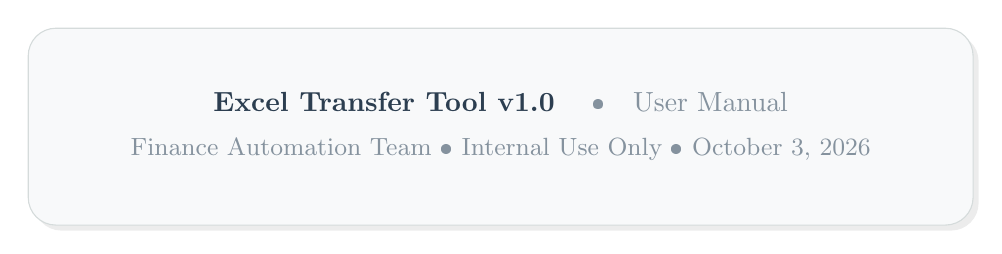
\begin{tikzpicture}
\node[draw=MidGray,fill=SoftGray,rounded corners=10pt,
      minimum width=12cm,minimum height=2.5cm,
      drop shadow={shadow xshift=2pt,shadow yshift=-2pt,opacity=0.15},
      align=center] {%
    \textcolor{PrimaryBlue}{\textbf{Excel Transfer Tool v1.0}}
    \quad\textcolor{MutedText}{\textbullet}\quad
    \textcolor{MutedText}{User Manual}\\[4pt]
    \textcolor{MutedText}{\small Finance Automation Team \textbullet\ Internal Use Only \textbullet\ \today}};
\end{tikzpicture}
\end{center}

\end{document}








